% =============================================================================
\section{Day and Night}
A 24-hour clock runs at one game hour per 20 s (keys change the speed, pause it or jump between day and
night). The sun direction is computed from the hour:
\[
a=\frac{hour-6}{12}\pi,\qquad \mathbf{s}=\operatorname{normalize}(0.95\cos a,\ \sin a,\ 0.42),\qquad
\mathbf{m} = \operatorname{normalize}(-0.8\,s_x,\ -s_y,\ 0.3).
\]
The sun rises in the east ($+x$) at 6:00, is highest at noon and sets at 18:00; the moon $\mathbf{m}$ is on the
opposite side. All other values are blended from the sun height $s_y$: the sky zenith and horizon colours (with an
orange glow near sunrise and sunset), the sun colour, the ambient light, the fog colour and density, the cloud
colour and the exposure. The night factor
\[
\nu = 1-\mathrm{smoothstep}(-0.14,\,0.10,\,s_y)
\]
shows the stars and the moon, switches on the street lamps and the car headlights and wakes up the fireflies.
\Cref{fig:daytimes} shows the same view at four times of day.

% =============================================================================
\section{Textures}
\subsection{Procedural textures}
All 25 textures are generated at start-up from \emph{value noise}: random values on a grid are smoothly
interpolated, and several octaves are added (fractal Brownian motion):
\[
\mathrm{fbm}(\mathbf{p}) = \frac{\sum_{i=0}^{k-1} 0.5^{i}\,\mathrm{noise}(2^{i}\mathbf{p})}{\sum_{i=0}^{k-1}0.5^{i}} .
\]
The noise wraps around at the texture border, so the textures tile without seams. Patterns are built on top of it:
rows of bricks with mortar, wooden planks with grain $\sin(6v+\text{noise})$, tiles with grout, marble veins, woven
fabric, bark ridges, and \emph{cut-out} textures (leaves, grass, fern, palm frond, flowers, vine) whose alpha
channel marks the shape of the leaf.
\begin{figure}[H]\centering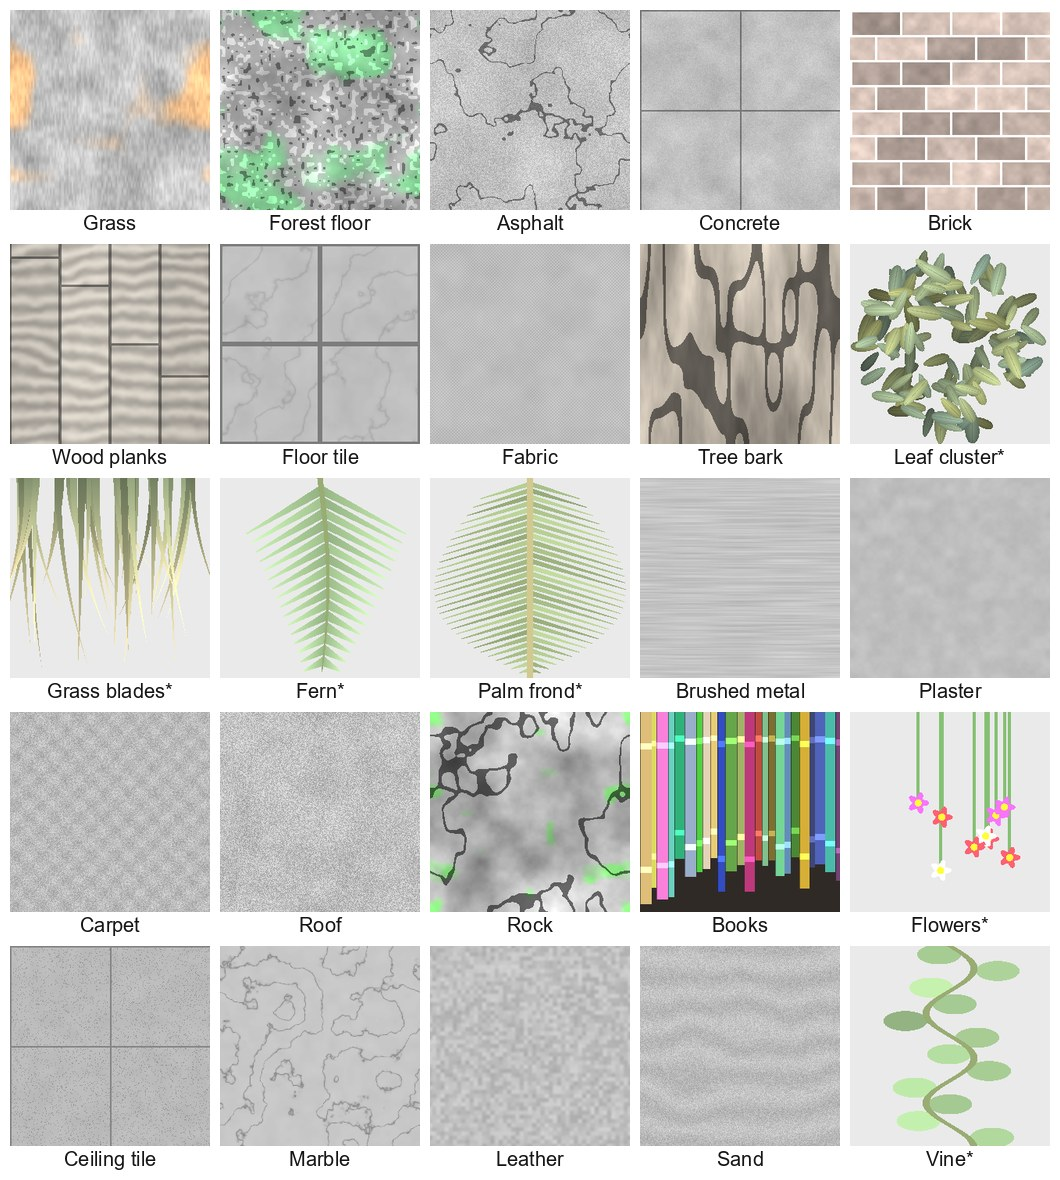
\includegraphics[width=0.9\linewidth]{textures}\caption{All procedural textures ($*$ = cut-out; light grey marks the transparent part).}\end{figure}

\subsection{Texture mapping}
\begin{itemize}
  \item All textures are layers of one \texttt{GL\_TEXTURE\_2D\_ARRAY} ($256\times256$, mip-maps, $4\times$
        anisotropic filtering). An instance only stores a layer number, so a texture change never breaks an
        instanced draw call.
  \item A texture stores a \emph{detail} value, and the final colour is $k_d = \text{colour}\times 2\cdot\text{texel}$,
        so the same brick texture works for any brick colour.
  \item \textbf{Object-space box mapping}: the shader selects the plane of the largest component of the local
        normal $\mathbf{n}_\ell$ and multiplies the local position $\mathbf{p}_\ell$ by the object's scale and the number of
        repeats per metre $\rho$:
        \[
        (u,v) = \rho\cdot\begin{cases}(x_\ell,\ z_\ell) & |n_y|\ge|n_x|,|n_z|\\ (z_\ell,\ y_\ell) & |n_x|\ge|n_z|\\ (x_\ell,\ y_\ell) & \text{otherwise}\end{cases}
        \]
        A 10 m wall therefore shows ten times more bricks than a 1 m box, without texture coordinates in the mesh.
  \item Cut-out cards use their mesh texture coordinates, and pixels with $\alpha<0.5$ are discarded, also in the
        shadow pass, so leaves cast leaf-shaped shadows.
  \item The terrain blends lawn grass and forest floor with a large-scale noise and the distance from the clearing.
\end{itemize}

% =============================================================================
\section{Shadows}\label{sec:shadows}
Shadows use \textbf{shadow mapping} (\Cref{fig:shadowidea}).
\begin{enumerate}
  \item \textbf{Depth pass}: the scene is drawn from the sun with an orthographic camera ($\pm32$ m around the
        player, a $2048\times2048$ depth texture, about 3 cm per texel). Only the depth is stored.
  \item \textbf{Main pass}: every pixel is transformed into the light's space with a small offset along its normal,
        \[
        \mathbf{p}_{L} = P_L\,V_L\,(\mathbf{p}+0.05\,\mathbf{N}),\qquad (u,v,z) = \tfrac12\,\mathbf{p}_L/w_L + \tfrac12,
        \]
        and compared with the stored depth $z_{map}(u,v)$: the pixel is lit if $z - b \le z_{map}$, with the
        slope-scaled bias $b = 0.0006+0.0012(1-\mathbf{N}\cdot\mathbf{L})$.
  \item \textbf{Percentage-closer filtering}: five hardware-compared samples around $(u,v)$ (the centre counted twice)
        are averaged, $s=\frac16\sum_k w_k\,[z-b\le z_{map}(u_k,v_k)]$, which gives soft shadow edges.
\end{enumerate}
The shadow camera moves only in whole texels along its own axes and the light direction used for shadows changes
in steps of $0.5^\circ$, so shadow edges do not shimmer when the camera or the sun moves. Glass, grass and other
small details do not cast shadows.
\begin{figure}[H]
\centering
\begin{minipage}{0.42\linewidth}
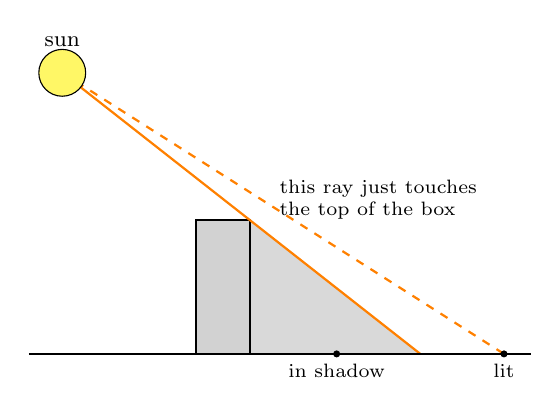
\begin{tikzpicture}[scale=0.85]
\fill[black!15] (2.8,0) -- (5.35,0) -- (2.8,2) -- cycle;
\draw[thick,fill=gray!35] (2,0) rectangle (2.8,2);
\draw[orange,thick] (0,4.2) -- (5.35,0);
\draw[orange,thick,dashed] (0,4.2) -- (6.6,0);
\draw[fill=yellow!60] (0,4.2) circle (0.35) node[above=6pt,font=\footnotesize]{sun};
\draw[thick] (-0.5,0) -- (7,0);
\fill (4.1,0) circle (1.5pt) node[below,font=\scriptsize]{in shadow};
\fill (6.6,0) circle (1.5pt) node[below,font=\scriptsize]{lit};
\node[font=\scriptsize,align=left,anchor=west] at (3.1,2.3) {this ray just touches\\the top of the box};
\end{tikzpicture}
\end{minipage}
\begin{minipage}{0.4\linewidth}
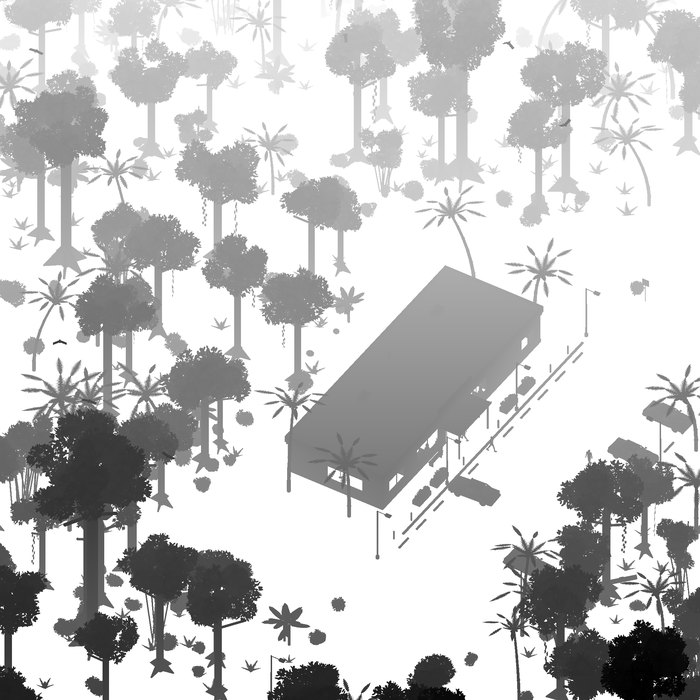
\includegraphics[width=\linewidth]{shadow_map}
\end{minipage}
\caption{Left: the principle of shadow mapping. Right: the depth image seen by the sun (darker = closer).}\label{fig:shadowidea}
\end{figure}
\begin{figure}[H]
\centering
\begin{subfigure}{0.49\linewidth}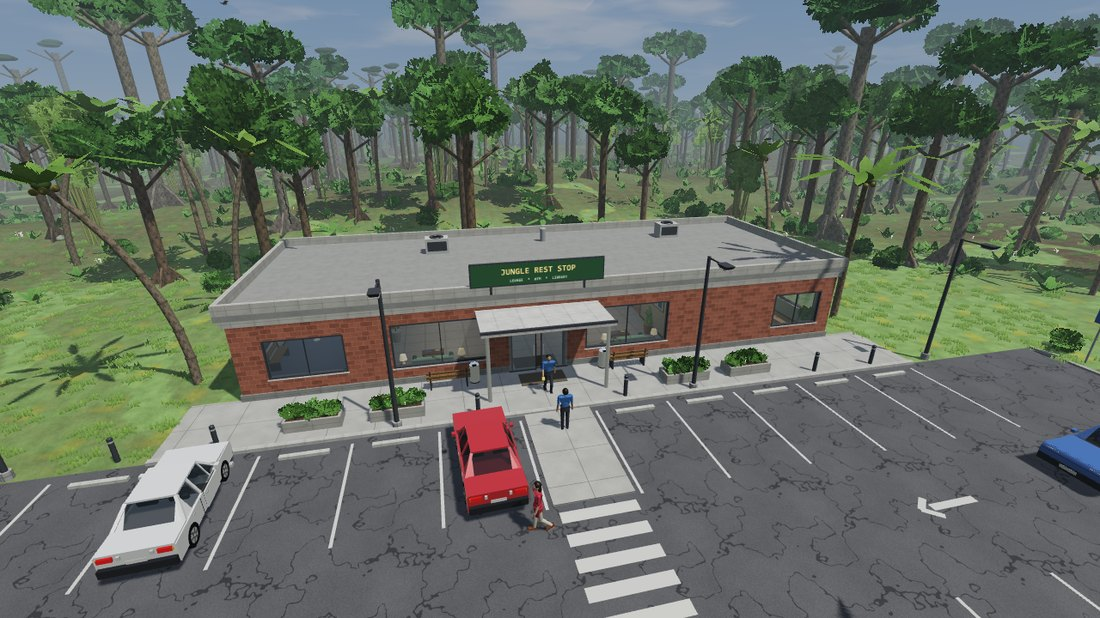
\includegraphics[width=\linewidth]{ext_day}\caption{Shadows on}\end{subfigure}
\begin{subfigure}{0.49\linewidth}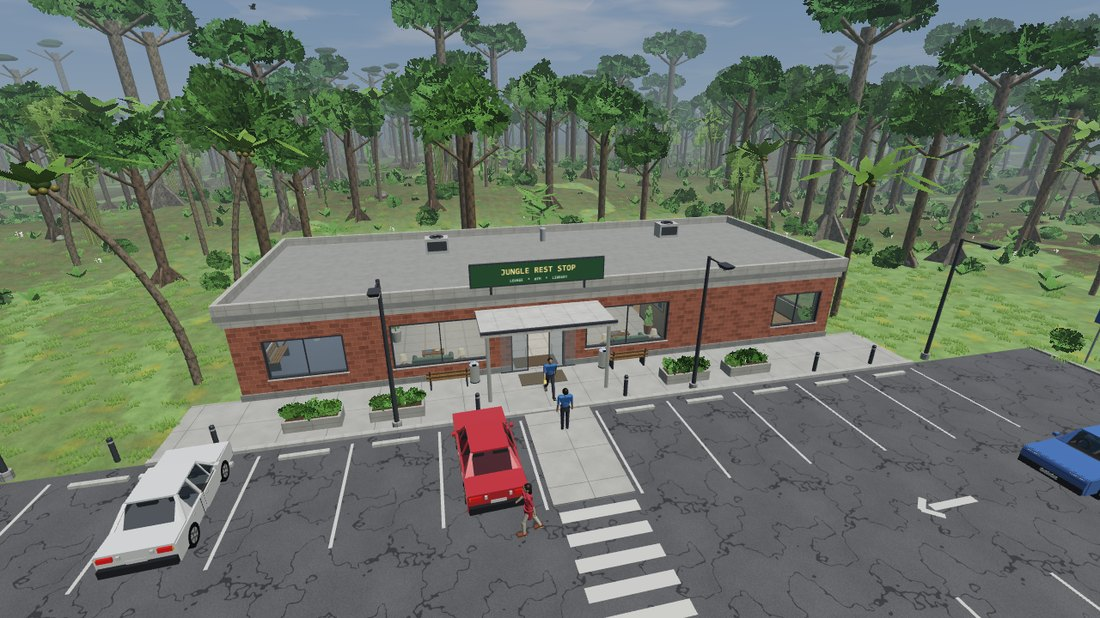
\includegraphics[width=\linewidth]{ext_day_noshadow}\caption{Shadows off}\end{subfigure}
\caption{Shadows show where objects touch the ground and give the scene depth.}
\end{figure}

% =============================================================================
\section{Sky, Fog, Tone Mapping and Wind}\label{sec:sky}
\begin{itemize}
  \item \textbf{Sky}: one full-screen triangle. For each pixel the view ray $\mathbf{d}$ is rebuilt with the inverse
        view-projection matrix. The colour is $\text{mix}(horizon, zenith, h^{0.55})$ ($h$ = height of the ray), plus a
        sun disc $\max(\mathbf{d}\cdot\mathbf{s},0)^{900}$ with a glow, a moon, twinkling stars (a hash on a 3D grid)
        and moving clouds (4-octave noise projected on a sky plane).
  \item \textbf{Fog}: the colour is blended towards the horizon colour with
        \[
        f = 1-e^{-(d\rho)^{1.5}},\qquad C' = (1-f)\,C + f\,C_{fog},
        \]
        where $d$ is the distance and $\rho$ the density. It hides the end of the world and gives a humid look; it is
        denser at night and thinner when the camera is high up.
  \item \textbf{Tone mapping}: $C' = 1-e^{-C\cdot exposure}$ keeps bright lamps from turning flat white. The exposure
        rises at night.
  \item \textbf{Wind}: leaves and grass sway in the vertex shader. The offset grows with the height inside the shape:
        $\Delta x = 0.05\,h\,\min(s_y,2.5)\sin(1.7t+0.35x+0.27z)$. The aquarium plants use the same rule as a water current.
\end{itemize}

% =============================================================================
\section{Basic Mode and Enhanced Mode}
\textbf{B} (or the on-screen button) switches between the modes; \textbf{T}, \textbf{G} and \textbf{F} switch
textures, shadows and fog one at a time.
\begin{table}[H]
\centering\small
\begin{tabular}{@{}lcc@{}}
\toprule
Feature & Basic & Enhanced \\ \midrule
Basic shapes, transformations, all objects & yes & yes \\
Blinn--Phong lighting with all lights, Phong shading & yes & yes \\
Procedural textures & -- & yes \\
Shadow mapping (PCF) & -- & yes \\
Fog & -- & yes \\
Sky with sun, clouds, stars & gradient & yes \\
Wind animation & -- & yes \\
Tone mapping & clamp & exponential \\
\bottomrule
\end{tabular}
\end{table}
\begin{figure}[H]
\centering
\begin{subfigure}{0.49\linewidth}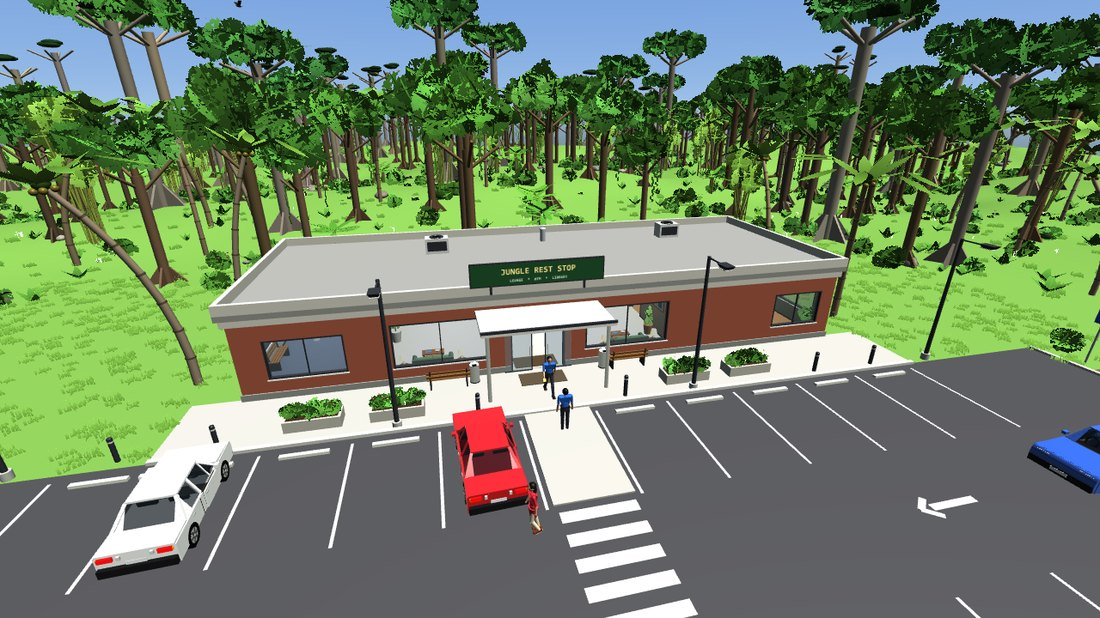
\includegraphics[width=\linewidth]{ext_day_basic}\caption{Basic}\end{subfigure}
\begin{subfigure}{0.49\linewidth}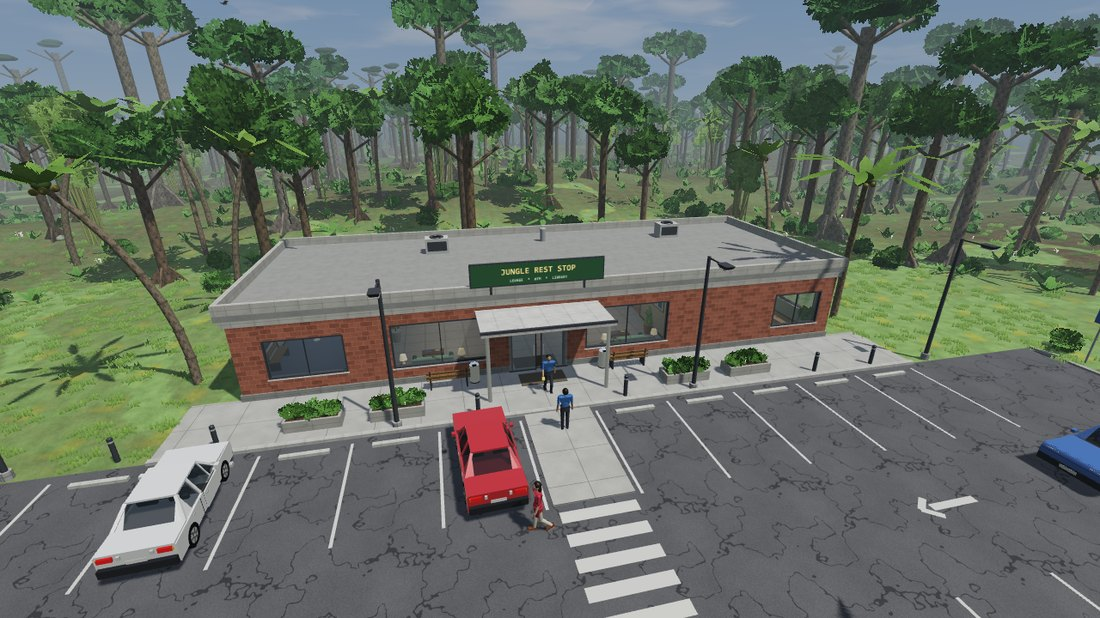
\includegraphics[width=\linewidth]{ext_day}\caption{Enhanced}\end{subfigure}
\begin{subfigure}{0.49\linewidth}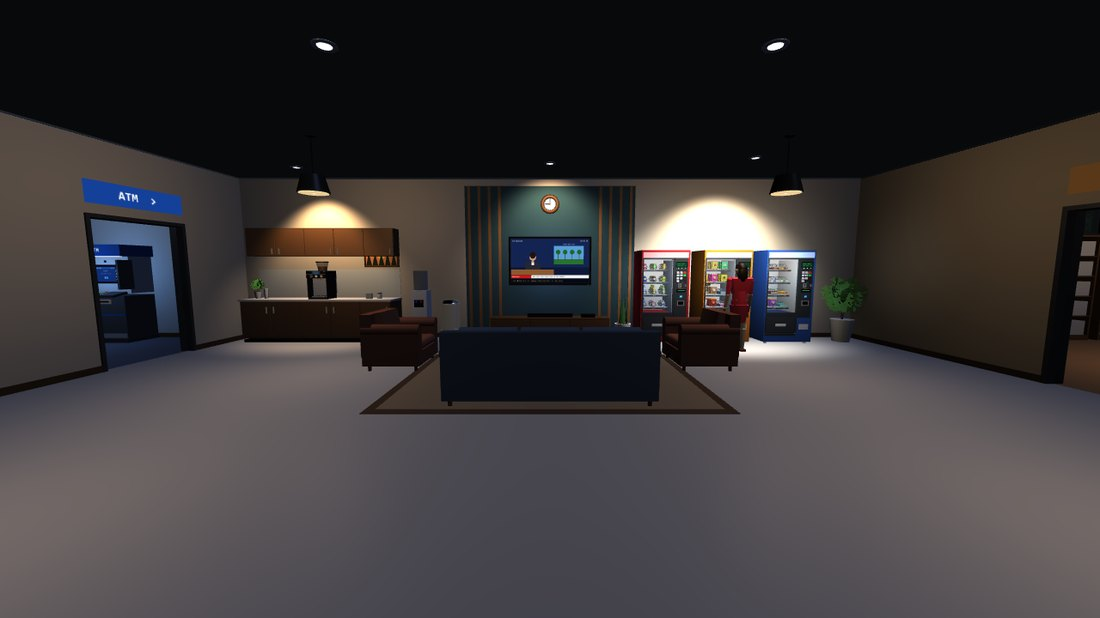
\includegraphics[width=\linewidth]{lounge_night_basic}\caption{Basic (interior)}\end{subfigure}
\begin{subfigure}{0.49\linewidth}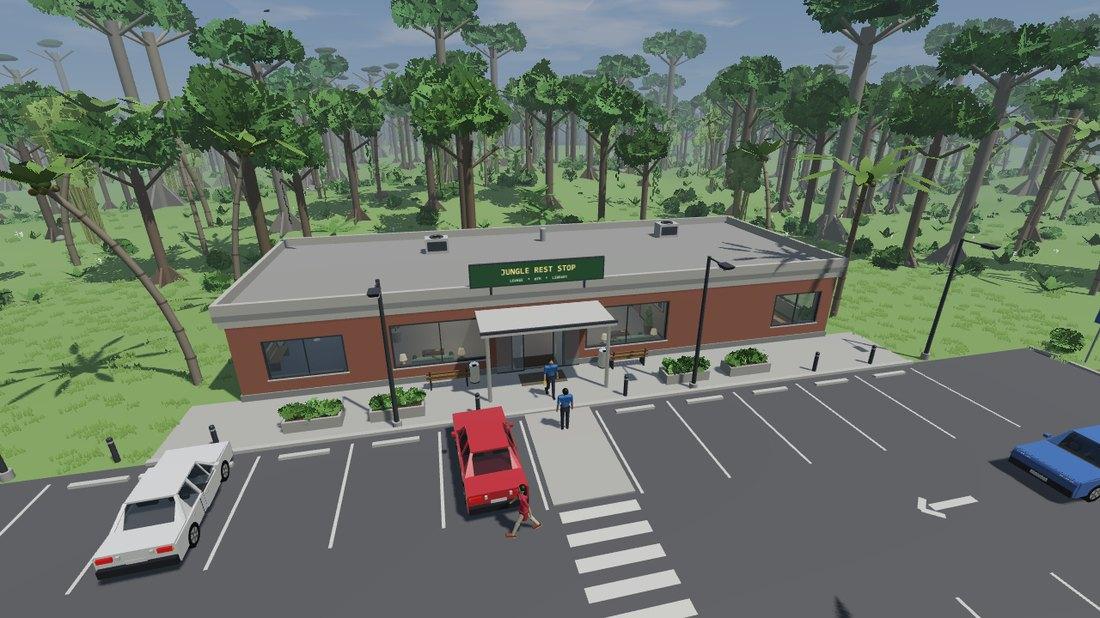
\includegraphics[width=\linewidth]{ext_day_notex}\caption{Enhanced without textures}\end{subfigure}
\caption{Basic and Enhanced rendering.}
\end{figure}
